%!TEX root = ./RoCKIn-D-2.1.6.tex

%--------------------------------------------------------------------
%--------------------------------------------------------------------
\subsection{Planning and Scheduling Functionality}
\label{ssec:PlanningScheduling}

%N youBot platforms (given by the organizer), driving from central station to several spots in the arena and set a flag "object collected/distributed". This avoids the problem if a team has a good scheduler, but problems with grasping occur

%--------------------------------------------------------------------
\subsubsection{Functionality Description}
\label{sssec:PlanningSchedulingDescription}

This functionality benchmark has the objective to test planning and scheduling capabilities of teams. 
It is important to separate this functionality from almost every other influence. 
Therefore, the teams will be presented with several robot platforms containing control software from the organizer.
The platforms will have no robot manipulators and will only simulate grasping and collection of objects.
Thereby it is possible to exclude possible time delays, which are not caused by the team, but e.g., by grasping failures of real objects.
The platforms movements are then to be scheduled by the team's software and shall drive through several spots in the environment to simulate collecting or delivering of objects.
Collecting is simulated by stopping for a while (can vary from one up to ten seconds) at the particular location (the duration of the stop will be consistent for all the teams).

%--------------------------------------------------------------------
\subsubsection{Feature Variation}
\label{sssec:PlanningSchedulingVariation}

% It is possible to simulate a delivery or a collection of parts.
The number of available platforms can vary from one up to three platforms.
The number of demanded sets of objects can vary from one up to 4 sets (different and more of one kind).

%--------------------------------------------------------------------
\subsubsection{Input Provided}
\label{sssec:PlanningSchedulingInput}

The team is provided with several virtual lists of objects: e.g. A (A1, A2, A3, A4), B (B1, B2, B3, B4, B5, B6, B7), C (C1, C2, C3, C4, C5) as well as the location(s) of each object in the test bed.
One object can possibly have multiple storage locations.
The start positions of platforms is also known to the team.
The platform control software includes a prompt which displays the objects already collected (see Figure \ref{fig:PlanningandSchedulingDisplay}).
%
\begin{figure}[!htbp]
  \begin{center}
    \scalebox{1.0}[1.0]{
      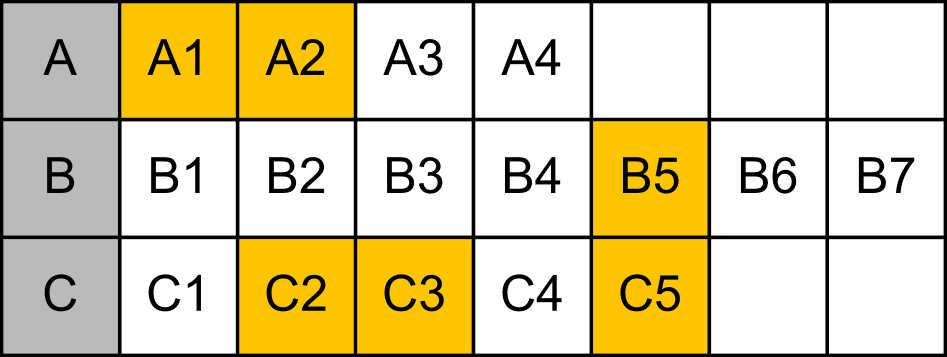
\includegraphics[width=\linewidth,angle=0]{pics/workObjects/PlanningDisplay}
    }
    \caption{Scheme of display mounted on each platform to visualize status of collected virtual objects. Sets of objects (A,B,C), objects (1,2,3,...) and already ``collected'' objects marked orange.}
    \label{fig:PlanningandSchedulingDisplay}
  \end{center}
\end{figure}
%
Workstation \# 5 serves as a dropping location.
Additionally, the rules and conditions that apply for several objects are provided:
%
\begin{itemize}
\item Objects within each list are ordered, i.e.~they should be collected by the robot in order (e.g., B1 needs to be collected before B2)

% there are some objects in a set of objects list that have to be collected before others (e.g., B5 needs to be collected before B2)
% \revtodo{GF: I suggest to change the above into "object within each list are ordered, i.e. they should be collected by the robot in order (e.g., B1 needs to be collected before B2)". This makes the scoring clearer.}

\item Some objects have multiple storage locations and multiple objects can be stored at one location (e.g., a shelf containing several containers with different objects). Therefore, in case of a blocked location, the robot needs to decide whether to wait or proceed with the same object in another location more far away (or collect the next object from a different set and return again).
\item Sets of objects can have different priorities (e.g., if set A has a higher priority than set B it has to be delivered, entirely, before set B).
%\item only complete sets can be delivered to workstation \# 5.
\end{itemize}

%--------------------------------------------------------------------
\subsubsection{Expected Robot Behaviour or Output}
\label{sssec:PlanningSchedulingOutput}

Expected behavior here relies to organizers robot platforms. 
The robots start from the central station and are commanded through the planning and scheduling software of the team.
The platforms should drive by and by to the demanded spots in the arena.
The platforms should also go to workstation \# 5 as planned by the team's software to ``empty'' their load.
During the execution of the task the control software from the team will monitor the execution of the benchmark and possibly issue new plans according to the current situation.
When the test is finished the platforms should stop at the central station again.

% \revtodo{MM I would add: During the execution of the task the control software from the team will monitor the execution of the benchmark and possibly issue new plans according to the current situation.}

%--------------------------------------------------------------------
\subsubsection{Procedures and Rules}
\label{sssec:PlanningSchedulingProcedures}

Every run of this functionality benchmark will be preceded by a safety-check similar to that described for the task benchmark procedures. 

All teams are required to perform this functionality benchmark according to the steps mentioned below. During the first two days of the competition, all teams are required to repeat it (2 times in a row on day 1 and 2 times in a row on day 2). On the third day, only a selected number of top teams will be allowed to perform it. Maximum time allowed for one functionality run is 10 minutes.

% \revtodo{MM: does the previous sentence make sense?}
%
\begin{description}
\item[Step 1] The central scheduler defines several sets of objects, that have to be collected.
\item[Step 2] The teams software pre-plans the scheduling of platforms.
\item[Step 3] The team's software sends commands to platforms, receives feedback and tentatively re-plans, if apparently platforms are blocking each other or priority conditions are violated.
\item[Step 4] The team's software receives feedback from platforms, when they are ready with collecting and can drop their load at workstation \# 5. The platforms return status of display (means objects already collected)
\end{description} 
%

%--------------------------------------------------------------------
\subsubsection{Acquisition of Benchmarking Data}
\label{sssec:PlanningSchedulingData}

During the execution of the benchmark, the following data will be collected\footnote{In the following, `offline' identifies data produced by the robot that will be collected by the referees when the execution of the benchmark ends (e.g., as files on a USB stick), while `online' identifies data that the robot has to transmit to the testbed during the execution of the benchmark. Data marked neither with `offline' nor with `online' is generated outside the robot. NOTE: the online data should also be displayed by the robot on its computer screen, for redundancy purposes, in case problems with wireless communications arise.}:
%
\begin{itemize}
\item Original plan generated by the scheduler and each new plan generated; [offline]
\item The current situation in terms of collected items and blocked robots;
\item Time at which each object of each list has been picked up;
\item Time at which each object of each list has been delivered to the destination;
\item Time at which the last item of each list has been delivered to the destination.
\end{itemize}
%
This list will be kept open so as to receive further suggestions from stakeholders.
Formats and interfaces for the transmission of internal robot data will be provided to the teams well in advance of the Competitions.

%--------------------------------------------------------------------
\subsubsection{Scoring and Ranking}
\label{sssec:PlanningSchedulingScoring}

Scoring is based on the following criteria:
%
\begin{itemize}
\item Number of completed lists of objects\footnote{A list is \textit{completed} when the last item of it is delivered to the destination.};
\item Order in which the lists have been completed;
\item Order in which the objects of each list have been delivered;
\item Time for the completion of all lists, if less than the maximum allowed for the benchmark.
\end{itemize}
%
Correct ordering, according to priority, between completed lists is considered as essential, and items of lists completed out of priority order are ignored. For instance, if list B is completed before higher-priority list A, all the items of B are considered as not delivered and do not contribute to the score.

The score of a team is given by the following elements:
%
\begin{enumerate}
\item Number of lists completed. A higher number of completed lists is preferred.
\item Ordering in which elements of each completed list have been delivered. Correct ordering of the items is preferred. For each list, scoring follows the Levenshtein distance between the required list of items (e.g., $\left[A1\;A2\;A3\;A4\;A5\right]$) and the list of items actually delivered (e.g., $\left[A1\;A3\;A2\;A5\right]$).\footnote{This distance takes into account also out of order execution and missing items (the last property is only useful for incomplete lists, which will be considered later).}
\end{enumerate}
%
The scoring elements above are prioritized: whatever the ordering of elements in completed lists, a robot which has completed a higher number of lists always gets a higher score. %When teams have completed the same number of lists the ranking is derived by the ordering of the list's elements.

Between teams that obtain the same score according to the preceding scoring elements and completed all the lists, ranking is defined according to the time of completion of the last-completed list.
Between teams that obtain the same score according to the preceding scoring elements but did not complete all the lists, ranking is defined by the ordering of the elements of incompletely delivered lists, evaluated using the Levenshtein distance.

% \revtodo{MM: the previous scoring is quite elaborated, we reserve to change it on the next rule book revision after a few simulations.}

%--------------------------------------------------------------------
% EOF
%--------------------------------------------------------------------
